%!TEX root = ../tese.tex
%!TEX encoding = UTF-8 Unicode

\chapter{The Shuttle Architecture}
\label{chapter:architecture}
This chapter describes the overall system architecture of Shuttle and outlines its central functional components. The main design goal is to help \ac{CSP} customers to recover from intrusions in their applications deployed in \ac{PaaS}. We consider three actors: the \ac{CSP}, which provides the platform, the \emph{tenants}, who deploy their applications in the platform, and the \emph{users}, who access the applications. Shuttle is a service designed to be offered by a \ac{CSP}.

We introduce the main requirements in Section \ref{sec:arch:requirements} and describe a generic \ac{PaaS} architecture in Section \ref{sec:arch:paas}. The remaining sections describe the architecture of Shuttle and discuss the main design choices.

\section{Requirements}
\label{sec:arch:requirements}
This thesis addresses the problem of providing an intrusion recovery service for applications deployed in \ac{PaaS}. Our overall goal is to \textit{make \ac{PaaS} applications operational despite intrusions}. More precisely, we aim to create a service, named Shuttle, to help \ac{PaaS} tenants to recover from the following problems in their applications:
\begin{itemize}
\item \textit{Software vulnerabilities:} non-authorized users compromise state by exploiting software vulnerabilities that allow invalid requests to be executed.
\item \textit{Malicious or accidentally corrupted requests:} users, authorized or not, compromise the application state accidentally or intentionally issuing valid requests.
\end{itemize} 




%attack example
For instance, two common attacks that can be used to compromise application state consist in: (1) attackers stealing valid users' credentials and using them to access their data; and (2) doing a \ac{SQL} Injection attack by mixing \ac{SQL} meta-characters with normal input and doing otherwise invalid queries to the database. Both attacks can be performed using apparently valid requests. Consequently, many prevention mechanisms fail to block them.

In order to achieve the above goals, the service shall meet the following requirements: 
\begin{itemize}
\item \textit{Remove intrusion effects:} Remove corrupted data at file system, database and application levels in the application containers and update affected legitimate actions. 
\item \textit{Remove selected malicious actions:} Help tenant to track the intrusion producing the set of actions affected by an externally provided list of malicious actions.
\item \textit{Support software update:} After recovery, the application state has to be compliant with the new version of the software.
\item \textit{Recover without stopping the application:} Recover the application without exposing users to application downtime.
\item \textit{Determinism:} Despite concurrent re-execution of requests, the result of re-execution is the same as the result of first execution if the application source code and requests remain equal.
\item \textit{Low runtime overhead:} The recording of operations or state for recovery purposes should have a negligible impact in the runtime performance.
\item \textit{\acs{NoSQL} database snapshot:} \acs{NoSQL} databases will have to be extended to support database snapshots, in order to reduce the recovery time.
\item \textit{\ac{PaaS} integration:} The source code of the application shall remains unmodified as much as possible. \ac{PaaS} developers do not need to install or configure Shuttle. Shuttle is built in a generic manner and it is reused in each deployed application.
\end{itemize}

Shuttle shall \textit{support software updates} to prevent future intrusions and allow operators to try new configurations or software versions without effects in the application behavior perceived by users. 


\section{Platform as a Service}
\label{sec:arch:paas}
\ac{PaaS} is a cloud computing model for automated configuration and deployment of applications in a cloud infrastructure \cite{Vaquero2008,Vaquero2011,Armbrust,Mell}. \ac{PaaS} enables developers to develop and deploy web applications into production fast by abstracting many details of the underlying infrastructure. Developers access the infrastructure resources, such as storage, through a set of services. These services are often pay-per-usage. \ac{PaaS} provides a deployment environment for a set of languages. 

%Bottom-layer: IaaS, VMs
Applications are deployed in one or more application servers, e.g., Tomcat or NodeJS. \emph{Containers} \cite{Lenk2009} hold these application servers and provide the required isolation level between the various applications. The word container is often used to refer to lightweight in-kernel resource (CPU, memory and device) accounting, allocation and isolation mechanisms like the \textit{Linux control groups} \cite{Menage2007}. These mechanisms isolate the process, network and file system used by applications that share the same operating system. They can run either directly on the host operating system or in a virtual machine. In this document, we use the word \textit{container or instance} to mean an isolated deployment unit that can be allocated from a resource pool by an orchestration engine. The deployment unit is created using an image and has storage attached. Therefore, our concept of container includes not only \textit{Linux control groups} like systems but also bare metal servers and guest operating systems running on top of hyper-visors, e.g., Xen \cite{xen}, KVM \cite{kvm}. Containers are managed directly or through an orchestration or IaaS system (e.g., OpenStack \cite{openstack}, \ac{AWS} \ac{EC2} \cite{aws}, Eucalyptus \cite{eucalyptus}, Omega \cite{omega}). Containers have one or more associated storage. When the container loads up, it loads an image onto its storage. The image contains, at least, the operating system and the \ac{PaaS} system in order to deploy the application in the container. 

%Components
In order to let Shuttle as generic as possible, we consider the following components of a minimal \ac{PaaS} architecture (Figure \ref{fig:paasArchitecture}):
\begin{itemize}
\item \textbf{Load balancer:} Routes user requests based on application location and container load.
\item \textbf{Instance controller:} Collects the container metering data and performs the configuration, tear-up and tear-down of containers in the instance.
\item \textbf{Cloud controller:} Manages the tear-up and tear-down of containers.
\item \textbf{Metering and billing}: Retrieves the metering data from each container. The load balancer uses this information to perform request routing while the cloud controller automatically decides when to scale.
\item \textbf{Containers:} The isolated environment where applications run.
\item \textbf{Cloud Instances:} The guest operating systems or bare-metal machine where the containers run.
\item \textbf{Authentication manager:} Provides user and system authentication.
\item \textbf{Database instance:} A single \ac{DBMS} shared, or not, between multiple applications. Most database middleware are built-on multiple containers to provide scalability and replication.
\item \textbf{Authentication manager:} Provides user and system authentication.
\end{itemize}

\begin{figure}
\centering
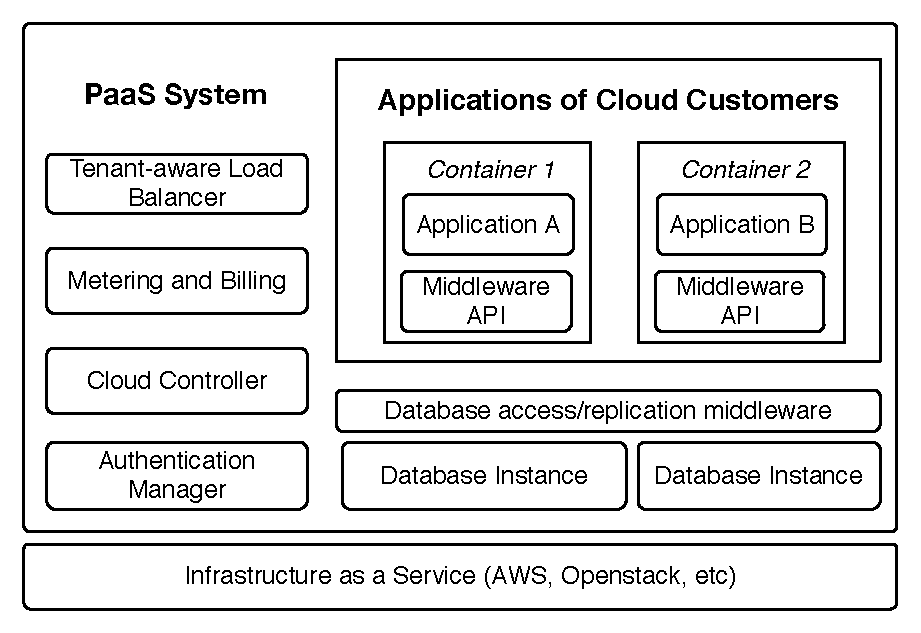
\includegraphics[width=100mm]{images/paas}
\caption{Generic \ac{PaaS} architecture}
\label{fig:paasArchitecture}
\end{figure}

\ac{CSP} also deploy the database management systems in containers. Their data is accessed as a service by the developers. Most of the applications deployed in \ac{PaaS} are designed to scale horizontally, i.e., to scale adding more containers. Therefore, the database and/or the session cookies often maintain the application state. The \ac{PaaS} systems are often integrated with code repositories and software development tools reducing the time deploy of applications in cloud environments. Users may access the website connecting to the load balancer via \ac{HTTPS}, which will decrypt the \ac{SSL} session and forward the unencrypted requests to application containers. As the traffic increases, the load balancer may become a performance bottleneck if the system does not provide enough resources to handle the user traffic.\\

We assume applications to store their persistent state only in databases. Shuttle's architecture can be extended to encompass object storage, for instance \ac{AWS} \ac{S3}. We do not consider a possible state stored in the filesystem because \ac{PaaS} applications are supposed to be scalable, thus the instances file system is frequently destroyed.

%%%%%%%%%%%%%%%%%%%%%%%%%%%%%%%%%%%%%%%%%%%%%%%%%%%%%%%%%%%%%%%%%%%%%%%%%%%%%%%%%%%%%%%%%%%
\FloatBarrier
\section{Shuttle Overview}
\label{sec:arch:overview}
Shuttle is an intrusion recovery service for \ac{PaaS}. It recovers from intrusions on software domain due to software flaws, corrupted requests, input mistakes and corrupted data in \ac{PaaS} containers (Section \ref{sec:arch:paas}). While previous works (Chapter \ref{chapter:related_work}) aimed to recover applications supported by a single database, Shuttle targets \ac{PaaS} applications deployed in multiple instances and backed by \acs{NoSQL} databases. Since typical \ac{PaaS} applications are designed to support high usage loads, our main contribution is a scalable intrusion recovery service that is transparent for application developers. 

%Summary
Shuttle is an automatic recovery mechanism based on the record-and-replay approach. Applications supported by Shuttle can operate in one of two states: \textit{normal execution} and \textit{recovery}. During \emph{normal execution}, Shuttle records the data required to recover the application afterward: it does periodic database snapshots, logs user requests and database operations. When an intrusion is identified, tenants use Shuttle to recover their applications staring the recovery phase.

The processes described in Section \ref{chapter:related_work} lead us to define \textit{how to remove the intrusion effects} and \textit{how to recover a consistent state}. During the \emph{recovery phase}, Shuttle removes the intrusion effects creating a branch of the system execution in which it loads a snapshot that contains an application state before the intrusion began. It builds a consistent state by replaying (re-executing), in the new branch, the legitimate requests logged during the \emph{normal execution}, performing either full or selective replay (Section \ref{sec:arch:selective_replay}). In the meantime, the incoming requests are executed in the previous branch. When ready, Shuttle sets the new branch as the single execution branch. \\



%PaaS
Shuttle aims to be integrated by CSPs into their \ac{PaaS} architecture as a novel service. Services provided in \ac{PaaS} are expected to be well-tested and available without setup because they are offered by \ac{CSP} and shared by multiple tenants. Our approach hides the Shuttle implementation and operation within the database and load-balancing \ac{PaaS} services. Shuttle components can be shared by multiple clients but the data of each client remains isolated. For sake of simplicity, we present Shuttle considering a single tenant implementation.

We consider a minimal \ac{PaaS} architecture to let Shuttle as generic as possible. We consider a client-server model in which clients access applications using the \ac{HTTP} protocol \footnote{Shuttle also supports HTTPS by ending the connections at the proxy.}. \ac{HTTP} requests are received by a load balancer that forwards them to web/application servers, which access a shared database. {PaaS} components are represented with solid line in Figure \ref{fig:shuttle_architecture}, while Shuttle components are represented with dashed line. \ac{PaaS} platforms with Shuttle have the following components:

\begin{itemize}
  \item \textit{Proxy:} Logs every \ac{HTTP} user requests, adds an unique mark to its header and forwards it to the load balancer. The proxy functionality might be part of the load balancer but conceptually it is a different component.% and currently it is also implemented separately.
  \item \textit{Load balancer:} Routes requests to different application servers taking into account their load (part of the \ac{PaaS} platform).
  \item \textit{Application servers:} The application (or web) servers are the components of the \ac{PaaS} platform that run the application logic. This logic uses a library to access the database service. Shuttle uses a \textit{database client interceptor} mechanism in this library to log the data items accessed per request.
  \item \textit{Database instances:} A set of database servers used to store the application persistent state. Shuttle includes in each instance  a \textit{database proxy} that logs the requests that accessed each data item and determines the dependencies between requests.
  \item \textit{Shuttle storage:} A scalable storage component that stores requests, responses and metadata.
  \item \textit{Manager:} Retrieves dependencies and coordinates the recovery process. 
  \item \textit{Replay instances:} A set of \ac{HTTP} clients that read previously executed requests from the Shuttle storage and invoke the application servers to re-execute the requests during the recovery process. The manager coordinates the worker instances.
  \end{itemize}


\begin{figure}[]
\centering
\subfloat[b][without Shuttle]{
    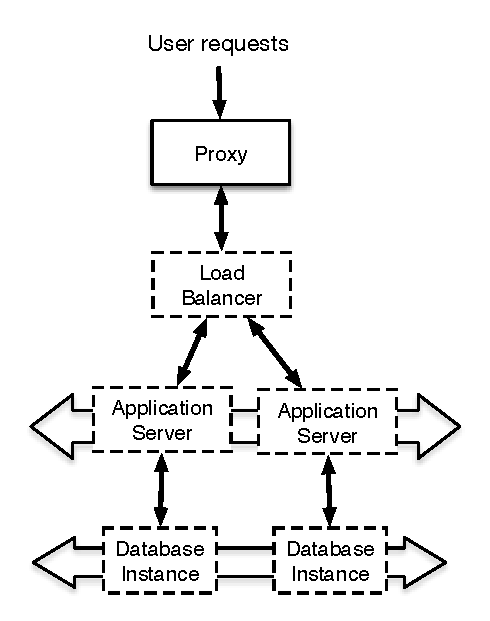
\includegraphics[width=0.35\linewidth]{images/architectureWithout}
}
\subfloat[b][with Shuttle]{
    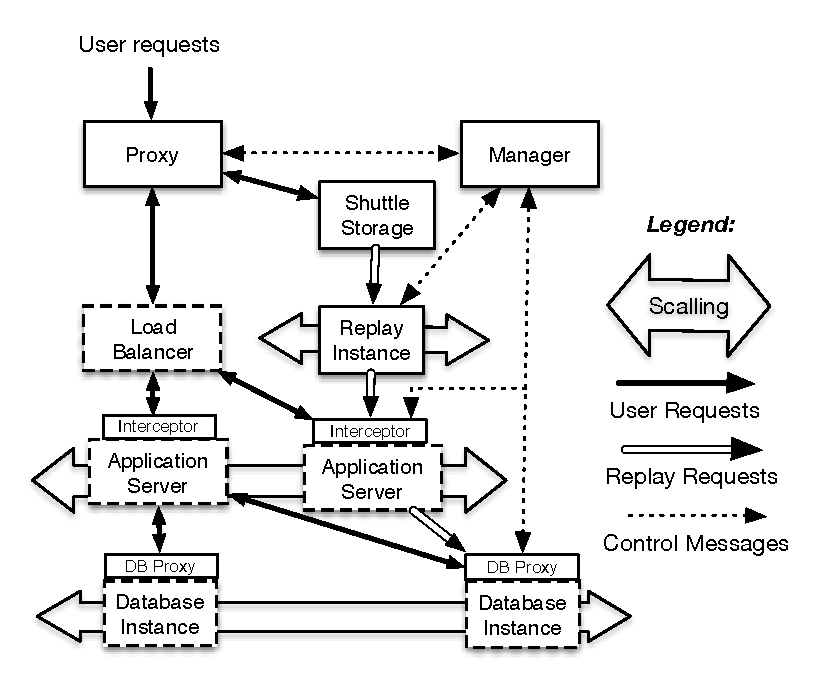
\includegraphics[width=0.55\linewidth]{images/architectureTiers}
}

\caption{Shuttle service architecture:The dashed line components are part of the \ac{PaaS} architecture. The proxy logs the user requests into the Shuttle storage. The manager coordinates the recovery process where the replay instances replay the user requests.}
\label{fig:shuttle_architecture}
\end{figure}
  

%Shuttle Storage
The \emph{Shuttle storage} keeps the content of the user requests and responses. Although we do not consider this aspect in the architecture, this store can be replicated to a remote site to allow tolerating catastrophic failures in a datacenter.


%trusted computing base
We consider the Shuttle components to be part of the trusted computing base since their integrity and availability are critical to recover the application state. We assume that intrusions tamper the application data, which is stored in the database, not the snapshots neither the stored requests. 

%Database
Unlike previous works, our design encompasses distributed databases (\acs{NoSQL}). These databases are designed to scale horizontally. Therefore, Shuttle can also be scaled by adding more database instances.

%How the architecture fits the PaaS
PaaS offerings are supported by a computing infrastructure, often provided as a service (IaaS model), able to scale the application allocating new instances on-demand or automatically, to maintain the quality of service despite demand oscillations. This elasticity  allows allocating replay instances and to scale the application to attend the requests issued by them during the recovery process. Due to the common pay-per-usage model, these resources are paid only when a recovery process occurs. The remaining cost of the service comes from storing client requests and database snapshots. Our design aims to optimize the available resources to reduce the recovery period and costs. 


%%%%%%%%%%%%%%%%%%%%%%%%%%%%%%%%%%%%%%%%%%%%%%%%%%%%%%%%%%%%%%%%%%%%%%%%%%%%%%%%%%%%%%%%%%%%%%%%%%%%%%%%%%%%%%%%%%%%%%%%%%%%
\section{Normal Execution}
\label{sec:arch:normal_execution}
Shuttle logs the data it needs to recover applications during the normal execution phase: user \ac{HTTP} requests, application \ac{HTTP} responses, database items accessed by each request and sequence of operations to each database item (Figure \ref{fig:normal_execution}). In this section, we describe the normal execution phase following the path that a request takes to be processed.

\begin{figure}
\centering
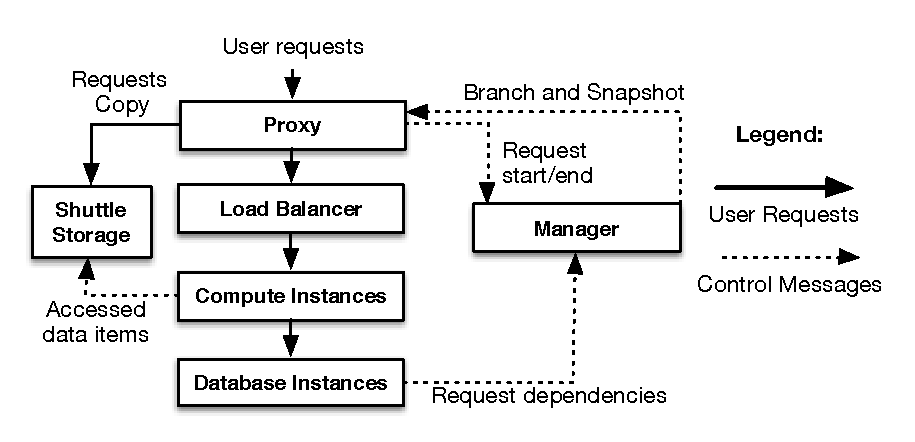
\includegraphics[width=130mm]{images/normalExecution}
\caption{Interaction between components during the normal execution}
\label{fig:normal_execution}
\end{figure}

%Proxy
The proxy intercepts all user \ac{HTTP} requests, except those to static contents (e.g., images), and adds a new header field named \ac{SRD}. Each \ac{SRD} contains three subfields: \ac{RID}, which is an unique timestamp; \emph{Branch} and \emph{Snapshot}, which define, respectively, the database branch and snapshot (Section \ref{sec:arch:snapshot}) and a \emph{restraint} flag, which is used to support runtime recovery (Section \ref{sec:arch:runtime_recovery}). 

The proxy also intercepts every application response, associates the response with the original request and adds a new timestamp to track the ending of the request execution. Requests, responses and their timestamps are stored in the \emph{Shuttle storage} using asynchronous I/O, which permits the operations to proceed before the transmission has finished. 

Requests are sent to the load balancer, which forwards the requests through the application instances according to their usage.


%Application instance
The application instances invoke the database service using the database client library. The database client library intercepts the operations, logs the accessed data items per request and stores this information in the \emph{Shuttle storage}. The database invocation is tracked at client side because the database may not be available or operations may fail.

%Database
On each database instance, the database proxy logs the operations' \ac{RID} and type. The sequence of operations to a data item defines its \emph{operation list}. Periodically, each database instance iterates the operation list of every data item to establish the dependencies between requests. Shuttle also performs snapshots periodically. The snapshot operation stores a new version of data item on the next write operation (Section \ref{sec:arch:snapshot}).


%Summary
In summary, every request-response pair is timestamped and logged by the proxy, the application instances the accessed data items per request, the database logs the sequence of operations per data item. The sequence of operations of each data item is kept in the database instance in which the data item is stored. The remaining data is stored in the \emph{Shuttle storage}, which can be located, or replicated, in a remote site to prevent catastrophic disasters rebuilding the application state using the requests and a previous snapshot. The manager retrieves, asynchronously, the requests' start and end timestamps, which are sent by the proxy, and their dependencies, which are collected by the database instances. Shuttle uses the information retrieved to generate the request dependency graph (Section \ref{sec:arch:dependencies}). 






%%%%%%%%%%%%%%%%%%%%%%%%%%%%%%%%%%%%%%%%%%%%%%%%%%%%%%%%%%%%%%%%%%%%%%%%%%%%%%%%%%%%%%%%%%%%%%%%%%%%%%%%%%%%%%%%%%%%%%%%%%%%
\section{Recovery}
\label{sec:arch:recovery}
%how we will recover?
The intrusion recovery process consists of three steps. The first step concerns the intrusion detection, in which tenants detect intrusions, suspicious behaviors or software flaws. Tenants may use automated tools such as \ac{IDS} \cite{itdb} to detect intrusions. The second step is vulnerability management in which vulnerabilities are identified, classified and mitigated. This work assumes that tenants identify the malicious requests (the subsequence of actions $A_{intrusion}$ whereby the attacker compromises the application) correctly and modify or remove them. Alternatively, tenants can provide an updated and vulnerability-free software version (Section \ref{sec:arch:detection}).
In addition, Shuttle provides several methods to help tenants to identify the malicious requests: determine the set of requests that accessed a set of affected database entries  after an estimated intrusion moment; group requests by user-session; compare database versions to check if the vulnerabilities are correctly mitigated.

The third step consists in removing the intrusion effects. Intrusions affect the application integrity, confidentiality and/or availability (Section \ref{sec:related:recovery}). Recovery from confidentiality violations is out of the scope of this document. However, we argue that the design of the applications should encompass cryptography techniques which may reduce data relevance and protect the data secrecy \cite{Maheshwari2000}.
Shuttle aims to recover applications from integrity violations, which often harm the availability. Shuttle can accomplish some of the goals of intrusion tolerance, keeping the application availability. Applications can keep providing a, possibly degraded but adequate, service during the intrusion recovery. Incoming requests are executed while the recovery process occurs without externalization to users (Section \ref{sec:arch:runtime_recovery}). In addition, Shuttle reduces the system downtime by reducing the time to recover when intrusions happen. Shuttle does not replace the intrusion prevention, detection and tolerance mechanisms, which are the primary lines of defense against attacks.\\

In order to remove the intrusion effects, Shuttle loads a database snapshot, which is selected by the tenant. The selected snapshot shall be previous to the intrusion moment in order to replace the value of every data item by a non-tampered value. Shuttle \textit{manager} orders the \ac{PaaS} controller to launch a new set of application instances and deploys an updated source code version, which may include code fixes. Then, the manager orders the database instances to load the selected snapshot (Section \ref{sec:arch:image_rejuvenation}). The application is intrusion-less now that the snapshot is previous to the intrusion and the application is redeployed on new instances. 

After, the manager initiates a set of \textit{replay instances} to replay the legitimate requests of the sequence of legitimate actions that happen after the snapshot, $A-A_{snapshot}-A_{intrusion}$. The replay instances retrieve a list of requests to replay and get the requests \ac{HTTP} package from the \emph{Shuttle Storage} (Figure \ref{fig:replay_execution}). Most \ac{PaaS} systems scale automatically and horizontally, i.e., they increment or decrement the number of containers based on the measurements of the containers usage. Therefore, the application-logic and data tiers scale to attend the requests from the replay instances, increasing the recovery speed.

The database separates the versions used by the replayed requests and the new requests, preventing the application from exposing a downtime. After the recovery process, the new requests are also forwarded to the recovered database version (Section \ref{sec:arch:runtime_recovery}).\\


The main version of Shuttle loads a previous database snapshot and replays every legitimate user request. An algorithm concerning selective replay is introduced in Section \ref{sec:arch:selective_replay}. \\

In the following sections, we discuss each of key process of the recovery phase in further detail.

\begin{figure}
\centering
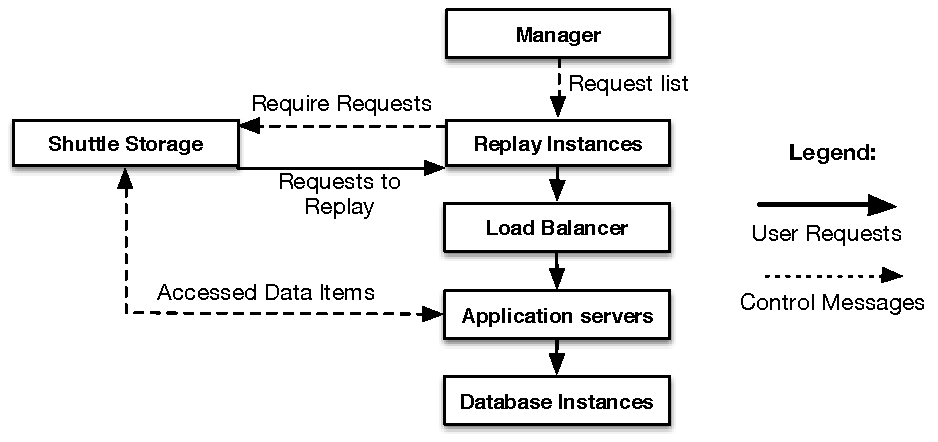
\includegraphics[width=110mm]{images/replayExecution}
\caption{Interaction between components during the recovery process}
\label{fig:replay_execution}
\end{figure}









%%%%%%%%%%%%%%%%%%%%%%%%%%%%%%%%%%%%%%%%%%%%%%%%%%%%%%%%%%%%%%%%%%%%%%%%%%%%%%%%%%%%%%%%%%%%%%%%%%%%%%%%%%%%%%%%%%%%%%%%%%%
\subsection{Intrusion and vulnerability correction}
\label{sec:arch:detection}
%how the damage is fixed?
The recovery process starts when intrusions are detected or the application software requires an update. Intrusion detection is out of the scope of this work. We assume that tenants, or system operators, detect one or more intrusions with the following sources:

\begin{enumerate}
\item User request (e.g. stolen user session)
\item External action: actions not logged by the proxy (e.g. ssh connection to the instances)
\end{enumerate}

Attacks may:
\begin{enumerate}
\item Tamper the database (e.g. adding new entries)
\item Tamper the container (e.g. changing the deployed application in the container)
\end{enumerate}

Shuttle supports the following actions to fix the exploited vulnerabilities:
\begin{enumerate}
\item Update the application software
\item Identify a set of tampered database entries
\item Add, modify or remove logged requests
\item Launch cleaned database or application server instances
\end{enumerate} 

Shuttle removes these effects of malicious actions redeploying the application in new containers and rolling back the database to a snapshot previous to the intrusion.

Attackers may use external actions to perform the intrusion, for instance gaining control of the instance to modify the database files. These actions are not recorded by Shuttle therefore they are not replayed and the application recovers a consistent state. We analyze several intrusion scenarios in Section \ref{sec:eval:accuracy}.\\


If tenants update the application software, they have to ensure that the application's interface remains compatible with the requests that will be replayed. Alternatively, tenants may update the entries in the database and provide a script to modify the requests make them compatible with the new \ac{API}. 

If the database is tampered using user requests, the tenant has to identify the malicious user requests. In addition,tenants can provide the set of suspicious database entries to Shuttle and it will resolve the set of requests that accessed the suspicious items after the estimated intrusion moment. Knowing the suspicious requests, the tenants shall use Shuttle to add, modify or remove the past requests to remove accidental or malicious behaves. \\

In summary, at the beginning of the intrusion recovery process, tenants shall ensure that:
\begin{enumerate}
    \item The software is correct: previous flaws are fixed, its \ac{API} is compatible with the requests and its behavior is the expected.
    \item The requests, which are selected to replay, are legitimate and their dependencies are correct.
    \item The estimated intrusion moment is previous to the intrusion moment (the selected snapshot is intrusion free).
\end{enumerate} 


%%%%%%%%%%%%%%%%%%%%%%%%%%%%%%%%%%%%%%%%%%%%%%%%%%%%%%%%%%%%%%%%%%%%%%%%%%%%%%%%%%%%%%%%%%%%%%%%%%%%%%%%%%%%%%%%%%%%%%%%%%%%
\subsection{Snapshot}
\label{sec:arch:snapshot}

%Why I need a snapshot? To reduce the work during replay.
Shuttle needs to remove intrusion effects. In Section \ref{sec:related:recovery}, we presented two mechanisms to do so: record the data item values or compensate the malicious actions. The first makes a copy of the data item value at a certain instant $t$, implying more storage resources. The second applies compensating actions to each action over the data item value after the instant $t$, which requires more computation resources to invert every action after $t$. However, the compensation mechanism requires the knowledge of the actions that revert the effects of the malicious actions. Moreover, if a malicious action is not recorded, then compensation mechanisms do not revert its effects. Since the set of operations is unknown and Shuttle aims to remove all intrusion effects, we perform snapshots by recording the value of the database items at a certain instant $t$ (first mechanism).\\

%What is a snapshot
A snapshot is a complete set of versions of every data item in the system from which data values can be read but to which updates are not made. Snapshots save the application persistent state at a certain moment. Unlike the selective undo approach, which only reverts the tainted data items (Section \ref{sec:arch:selective_replay}), the full replay approach loads a snapshot previous to the intrusion instant. This approach reverts every database item and removes the effects of any action that occurred after the snapshot creation. \\

%How it is useful?
The duration of the recovery process is mainly defined by the number of requests previous to the intrusion of the set, $A_{before}$. The snapshot mechanism avoids to replay every request from the beginning of the application, which can take too long. Shuttle requires not only a snapshot but also every action posterior to the snapshot instant. Therefore, Shuttle keeps every user request posterior to the oldest stored snapshot instant. The snapshot period defines the usage of storage and computation resources. We argue that tenants can balance the costs of storage and computation resources by specifying a policy to perform the snapshot. The policy shall consider the rate of requests, the data written per request, the expected time to detect the failure and the application capability to provide an possible degraded service during the recovery period. \\

%What Shuttle needs to do?
Shuttle takes snapshots automatically and according to specified policies. It records the persistent state of the application, i.e., the database values, at a certain instant. The volatile state of the application, for instance its stack, is not stored as we consider the web servers to be stateless. \\


%Request consistent snapshots
Performing snapshots in distributed databases is not trivial since snapshots have to be consistent with the user requests.  We consider each user request may include multiple database operations, each of them to multiple database servers, without using transactions. Consequently, the sets of database operations of each user request cannot be aborted and do not have a global order. If Shuttle replays requests on a snapshot that contains part of the persistent state written by a request during its first execution, the replay will be inconsistent. The database must reflect the effects of a set of completed requests and not the results of partially executed requests. Therefore each snapshot shall be \emph{global request consistent} containing either all or none of the database updates made by every request.


We define \textit{request consistent global snapshot}: a snapshot is global request consistent if it records a state of the database which reflects the effect of a set of completed requests and not the results of any partially executed request. This concept derives from the notion of \emph{transaction consistent global checkpoint}: a checkpoint is a transaction-consistent global checkpoint if it contains all or none of the updates made by a transaction \cite{global-checkpoint}. Since most \acs{NoSQL} databases do not support transactions, we extend the concept of transaction to \textit{request transaction}. A request-transaction embraces all database operations performed due to the execution of a request. Unlike \ac{ACID} transactions, a request-transaction may not be possible to abort. In summary, Shuttle snapshots are request consistent: a snapshot contain all or none operations of a request.


%Log-oriented vs dump-oriented vs Fuzzy
Checkpointing algorithms for distributed databases can be classified as log-oriented and dump-oriented \cite{checkpoint-survey}. In the dump-oriented approach, the checkpoint is referred to as the process of saving the state of all data items in the database. In the log-oriented approach, periodically a dump of the database is taken and also a marker is saved at appropriate places in the log. When a failure occurs, the latest dump is restored and the operations on the log after the dump was taken is applied to the dump until the marker is reached to restore the database to a consistent state \cite{global-checkpoint}. We take the latest approach.\\


In addition, the snapshot mechanism shall be non-blocking: the processes shall not stop their execution while taking snapshots.  

%Straightforward solution
A straightforward way to take a request-consistent global snapshot is to stop processing new requests, waiting until the currently executing requests finish, then making a copy of each data item. However, this solution incurs on communication overhead to reach a globally inactive state and causes application downtime. Yet, this approach may fit applications that can be unavailable during a certain period, for instance, during a certain period of the night. \\


Kim and Park \cite{kim_checkpoint} propose an approach in which a coordinator broadcasts a checkpoint-request message to every database node. Each database node divides the transactions into two groups: before the checkpoint-request $T_p$ and after $T_f$. Updates of transactions in $T_p$ are flushed to the current database, while the ones in $T_f$ are flushed in a \emph{checkpoint area} (a temporary allocated storage area). When all transactions of $T_p$ are done, the checkpoint area is updated with items updated by transactions in $T_p$ but not by $T_f$. After, the rules of current database and checkpoint area are exchanged. The major drawback of this approach comes from updating the checkpoint area: the database is unavailable during the updating process.


%Our solution
Our solution leverages the existence of a single load balancer and, consequently, single proxy that adds a \ac{SRD} field to every request. Every \ac{SRD} contains a \ac{RID}, an unique and incremental identification of each request given by the instant when the request is retrieved. Every database operation is identified by the \ac{RID} of the source user request.

In order to create a snapshot, tenants define a future instant in time $t$ when the snapshot will occur. The instant, named \ac{SID}, identifies the request-consistent global snapshot. The manager passes the \ac{SID} to every database proxy.

Database proxies use the \ac{SID} to define the version of the data item used by the operations. Operations with \ac{RID} lower than the scheduled snapshot instant (\ac{RID} < \ac{SID}) access the version before the snapshot. Otherwise, the operations access the latest data item version. This mechanism splits requests to accomplish a request-consistent global snapshot, and allows tenants to schedule snapshots without application downtime. Figure \ref{fig:snapshots} illustrates the sequence of 7 database operations on the database item $x$ and 3 snapshots (excluding the base snapshot).

\begin{figure}
\centering
  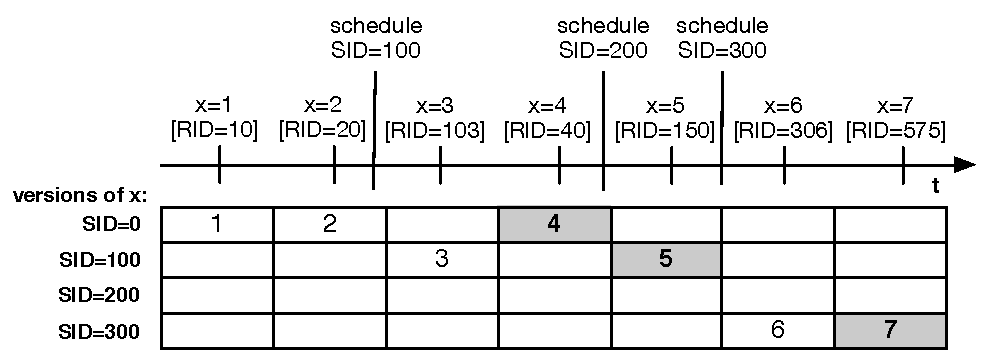
\includegraphics[width=130mm]{images/snapshots}
  \caption[Snapshot versions stored in the database]{Versions stored in the database during a sequence of 7 operations and 3 snapshots. The final values of the stored versions are contained in filled squares. The tenant schedules 3 snapshots on SID: 100, 200, 300.}
\label{fig:snapshots}
\end{figure}

In order to avoid to replay every database operation to obtain the snapshot, the snapshot mechanism shall create a database copy (dump). We avoid blocking the application to copy values using a copy-on-write and incremental method. When a data item is written for the first time in each snapshot, Shuttle creates a new version of the data item. Since a data item may not be written in every snapshot, e.g., $SID=200$ in Figure \ref{fig:snapshots}, we associate a \emph{version list} to every data item. A \emph{version list} tracks on which snapshots the data item has been written. In conclusion, the snapshot is an incremental mechanism because it does not require to duplicate data.\\
%The version list also contains read requests that did not succeeded, for instance when the data item does not exists, to avoid false positives. 


%Particular case
A snapshot might become inconsistent. For instance, Table \ref{tab:snapshot_caso_bicudo} represents the execution of two concurrent requests. Their normal execution is consistent. A snapshot with \ac{SID}=5 would contain [A1 = 11] and be a global request-consistent. However, if Shuttle loads the snapshot and replays the request 20, its first read operation reads A1 == 11 instead of A1 == 10. 


This particular case happens when a request with \ac{RID} greater than the snapshot instant \ac{SID} read a version belonging to the snapshot \ac{SID} and, after, a request with \ac{RID} lower than \ac{SID} overwritten that version. Storing a new version and adding a flag on the version list solves the problem. Nevertheless, we expect this to happen only in rare occasions.

%the  and every operation with \ac{RID} > \ac{SID} reads/writes the new version. Operations of requests with \ac{RID} > \ac{SID} that read the original value, for instance A = 10, are marked and read the old version during the replay. 
%in parallel during the transition period, i.e., when a request accesses the previous snapshot and other accesses the current snapshot. 


\begin{table}
\centering
\begin{tabular}{l|l|l}
\textbf{RID=10 (SID = 1)}     & \textbf{RID=20 (SID=15)}   & \textbf{Storage}\\ \hline
Write A=10                    & ~                          & A1=10  \\
~                             & Read A: A1==10             & A1=10  \\         
~                             & Write A=20                 & A1=10, A15=20 \\
Read A: A1==10                & ~                          & A1=10, A15=20 \\
~                             & Read A: A15==20            & A1=10, A15=20 \\
Write A=11                    & \textit{Completed}         & A1=11, A15=20 \\
\textit{Completed}            & ~                          & A1=11, A15=20 \\
\end{tabular}
\caption[Concurrent requests]{Concurrent requests: the snapshot instant is 15, the left request accesses data previous to the snapshot (A1) while the right accesses the latest (A15 or A1). }
\label{tab:snapshot_caso_bicudo}
\end{table}


%Discussion
Unlike the approach proposed by Kim and Park, our approach allows to record multiple snapshots keeping various data item versions and does not require to to copy the transactions.

The value of \ac{SID} must be known by every database instance before the execution of any request with $RID > SID$. If the \ac{RID} was determined by incremental request counter, then Shuttle would need to analyze the request rate and estimate the \ac{SID} value. However, the request rate can vary and the snapshot would fail. Notice that our mechanism does not require clock synchronization because the \ac{RID} is defined by the proxy timestamp and tenants can schedule a snapshot defining a future time instant. The period between the scheduled moment and the present must be bigger than the communication delay between the manager and the database instances. Consequently, we assume the communication between the manager and database proxies is synchronous: the messages are delivered within a fixed time.


%%%%%%%%%%%%%%%%%%%%%%%%%%%%%%%%%%%%%%%%%%%%%%%%%%%%%%%%%%%%%%%%%%%%%%%%%%%%%%%%%%%%%%%%%%%%%%%%%%%%%%%%%%%%%%%%%%%%%%%%%%%%
\subsection{Dependency Graph}
\label{sec:arch:dependencies}
%Dependency definitions
An application execution can be modeled as a set of actions and a set of objects. Actions read and write objects. An action $A$ is dependent from an action $B$ if $A$ reads an object's version written by $B$.

%why is relevant in general
Requests must be replayed in a consistent manner to obtain a consistent application after the replay phase. The request replay order must ensure that if the requests, application semantics and initial database values are the same, then the final database values are equal. For this propose, the dependencies between actions shall remain consistent: if during the first execution an action $A$ becomes depends on an action $B$ by an object $O$, then during the replay phase $A$ shall read the object $O$ only after $B$ updates the object $O$. Otherwise, $A$ may read a version different than the original version.

%related work and why it does not work in PaaS
Previous proposals, for instance \emph{in} \cite{goel}, leverage the request serialization provided by snapshot isolation in relational \ac{DBMS} to order the operations to replay. In contrast, \textit{Undo for Operators} \cite{undoForOperators} uses the application protocol knowledge to establish the dependency between requests and order them. However, accesses to \acs{NoSQL} databases are not globally serialized. Moreover, the data items accessed during the replay phase may change due to updates to the application semantics, request modification or multi-threaded execution. At last, the application semantics is unknown in advance since we want to support any application deployed on \ac{PaaS}. Taking that into account, we propose a novel approach.\\


%Rules
Shuttle tracks the dependencies between actions in a \textit{dependency graph}. A \emph{dependency graph} consists of nodes that represent requests and edges that establish dependencies between them (Figure \ref{fig:selectiveGraph}).  Dependencies between requests are established using the following rules: a request $R_A$ is dependent upon request $R_B$ if there is a data item $x$ such that $R_A$ reads $x$ and $R_B$ performs the latest update on $x$ before the read operation by $R_A$. Dependencies are transitive except when requests perform blind writes, i.e., requests write items without reading them first \cite{Ammann2002}. Therefore, the dependency graph is a mixed graph, if there is a dependency between $A$ to $B$, then there may be a dependency between $B$ and $A$.


%How Shuttle creates the dependency graph?
Previous solutions for relational databases extract the dependencies using a pre-defined, manually-created, per-transaction type template \cite{itdb}, or change the relational database management system code to extract read dependencies \cite{phoenix}. In contrast, Shuttle uses the database proxy to log the database accesses. Periodically, each database proxy traverses, in background, the \emph{operation list} of each data item to collect the new accesses and to generate the dependencies between requests. The Shuttle manager processes the dependencies to update the dependency graph. An alternative approach is to pull the dependencies from each database node only before the recovery process and generate the dependency graph when needed. 






%false positives: detected but not exist
The above method may lead to \emph{false positives}, i.e., to flag dependencies that do not exist. For instance, a request may read a data item but not use it to compute the written value, so there is no real dependency. Although tracking variables used by each request during its execution might solve this particular case \cite{goel}, it would require modifying the code interpreter (e.g., Zend Engine for PHP), which would constrain Shuttle to a set of specific languages. As our approach uses the dependencies to group the requests that can be executed concurrently, false dependencies imply a performance penalty but do not cause data loss or inconsistent state. On selective replay mode, the dependency graph is used to determine the tainted requests and the request that need to be replayed. Again, false dependencies only harm the performance.

When tenants use the dependency graph to determine the set of malicious requests, $A_{malicious}$, they shall take into account that false dependencies may lead to consider legitimate operations as malicious and, consequently, cause data loss.

%false negatives: not detected but exist
Complex queries on a relational database may lead to \emph{false negatives}, i.e. a dependency exists but is not detected. For instance when a read operation would have been executed on a deleted data item if this data item had not been deleted before the request execution \cite{Xie2008}. Therefore, legitimate transactions may have different output even when they were not affected by malicious execution during their original execution. Since user mistakes are often delete operations due to wrong query arguments, this is a relevant issue. 

In contrast with SQL queries that access the data items that match a query, the \ac{CRUD} interface of most key-value stores specifies, in a deterministic and apriori manner, the data item that will be accessed. Shuttle logs every access, even when the data items do not exist, keeping the \emph{operation list} of the deleted data items to track further operations.\\


%Cycles
%Each request may perform multiple database operations, each of them to multiple database servers, without defining a global \ac{ACID} transaction. 
Shuttle can not replay requests synchronously, i.e., waiting for the response to the previous request before sending the next. To replay the requests synchronously would not have only performance degradation but also lock the replay phase because requests, which have been originally executed in concurrently during the normal phase, may be depend on each other. Therefore, Shuttle replays requests asynchronously and, hence, concurrently. Two requests are executed concurrently if they are dependent from each other. For instance, Figure \ref{fig:inconsistency_db_order} represents the first execution of two requests that increment the variable $A$. The $Request 1$ depends on $Request 2$ and vice versa. 

%Ordering using operation list
Yet, re-execution of concurrent requests is not deterministic. User requests are processed concurrently using multi-threaded servers and the system messages, including database requests, do not have a delivering order. Therefore, the execution order of two concurrent requests is unknown. To deal with this issue, our novel approach uses the \emph{operation list} to turn the re-execution of concurrent requests deterministic. An \emph{operation list} is a sorted list that records the operations to a data item. During the replay phase, the operations to a data item must follow the order established by is operation list. For instance, in Figure \ref{fig:inconsistency_db_order}, the operation list of the data item $A$ is: $[Req1:Get, Req1:Put, Req2:Get, Req2:Put, Req1:Get, Req1:Put, Req2:Get, Req2:Put]$. {Req.~1} and {req.~2} are replayed concurrently but the result is consistent because the order is established by the operation list.

%Unlocking
During the recovery period, intrusions are removed and the application code is updated. This may cause requests to access different data items than in the first execution. Requests may not access the same sequence of data items or read/write the same content. If an operation contained in the operation list is not performed, the following operations to the data item are blocked and the request fails. To address this problem, at the end of each request execution, the \textit{database client interceptor} fetches the list of data items accessed by the request on its first execution and compares them against the ones accessed during the replay process. The database client library invokes the \emph{database proxy} with the data items that have not been accessed to unlock the operations of the remaining requests. 

For instance in Figure \ref{fig:inconsistency_unlock}, the $Request 1$ has a different replay execution performing $B = B \times 5$ instead of incrementing $A$. The second operation of {req.~2} is delayed until the end of the {req.~1} because it succeed the second operation of {req.~1} in the operation list. After the execution of {req.~1}, the database client interceptor unlocks the second operation of {req.~2}.\\

\begin{figure}[!htb]
\hspace*{-1cm}
\mbox{
  \subfloat[][Ordered by the operation list \label{fig:inconsistency_db_order}]{
      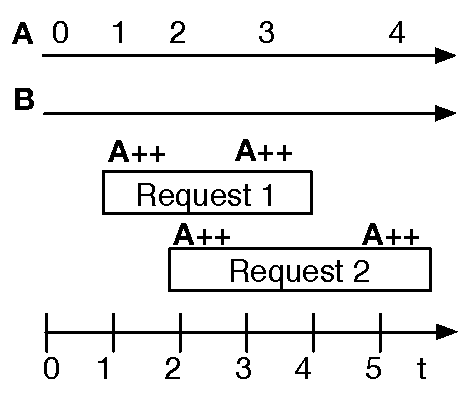
\includegraphics[width=0.25\linewidth]{images/inconsistency_db_order}
  }

  \subfloat[][Operation unlock \label{fig:inconsistency_unlock}]{
      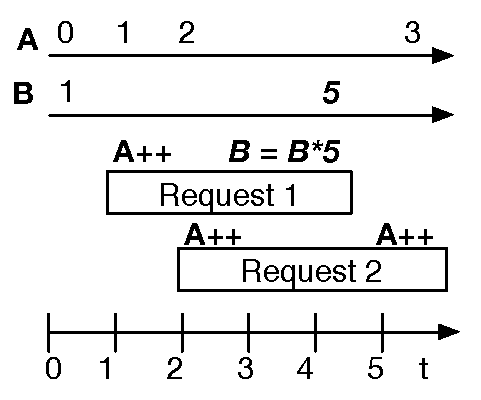
\includegraphics[width=0.25\linewidth]{images/inconsistency_unlock}
  }

  \subfloat[][Consecutive requests \label{fig:inconsistency_serial}]{
      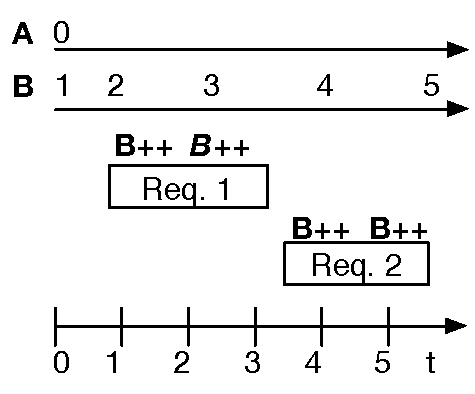
\includegraphics[width=0.25\linewidth]{images/inconsistency_serial}
  }

  \subfloat[][Conflict \label{fig:inconsistency_conflict}]{
      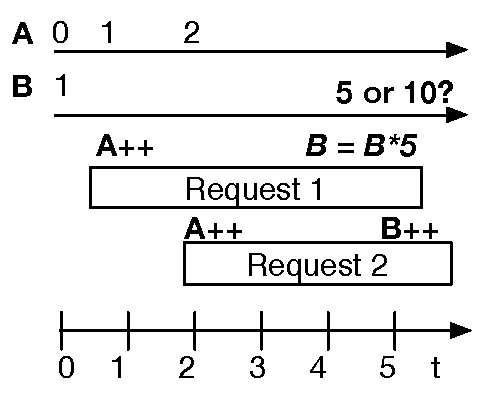
\includegraphics[width=0.25\linewidth]{images/inconsistency_conflict}
  }
}
\caption{Replay two requests with different re-execution}
\label{}
\end{figure}


%New dependencies during the recovery time
During replay there may be non-deterministic situations, whenever an access is not contained in the operation list. The most complex scenario during the replay is when two requests, originally executed in parallel, access different data items comparing with their first execution, establishing a new dependency. The result is unpredictable. Consider the possible re-execution in the Figure \ref{fig:inconsistency_conflict} where the {req.~2} increments $B$ simultaneously with {req.~1} performing $B = B \times 5$. The result is unpredictable because the {req.~1} may write before or after {req.~2}. Since both requests did not access the data item $B$ during their first execution, the operation list does not establish an access order. Therefore, the {req.~1} and {req.~2} may execute on a arbitrary order. The order of these requests is as deterministic as if during the first execution: the operation of \emph{req.~1} can execute before, between or after \emph{req.~2}.


%naive
A naive solution would be to detect the new dependency during the replay process, stop the process and start a new replay process in a new snapshot, including the new dependency.

%brown
Brown \textit{et al.} \cite{undoForOperators} propose the concept of \textit{verb} (Section \ref{sec:related:recovery_app}). A verb object encapsulates a single interaction (request/response) of the user and exposes an interface to establish the order between requests and their dependencies. However, tenants shall know the applications' operations to create the verbs defining: a commutativity test, an independence test, a preferred-ordering-test and an application-defined action to handle a inconsistency if the operation fails. Since Shuttle shall support any \ac{PaaS} application, the applications' semantics are unknown in advance. Therefore, this solution is not adequate.

%sorted log
A sorted-log, in which the accesses are sorted, for instance by \ac{RID}, would establish that operations must have a strict incremental order. However, operations with smaller \ac{RID} than the previous are aborted. For instance, the second operation of {req.~2} in Figure \ref{fig:inconsistency_db_order} would be aborted.

%sorting per start-end
An alternative solution consists on sorting the requests per \emph{start-end order}, instead of using the dependency graph. A request starts only after all requests with end lower than it ends. Dependencies between requests remain correct, since they are constrained by the \emph{operation list}. Thus the parallel requests are ordered and replayed in a similar manner to the first execution. Two serial requests can have distinct re-executions: if a request starts after the end of the previous. For instance in Figure \ref{fig:inconsistency_serial}, {req.~1} and {req.~2} can have distinct re-executions.

If two operations are re-executed concurrently, then their order is as deterministic as if they happen during the first execution. For instance in Figure \ref{fig:inconsistency_conflict}, the operation of {req.~1} $B = B \times 5$ is executed in parallel with the operations $B++$ of {req.~2}. The order of these requests is as deterministic as if during the first execution: the operation of {req.~1} can execute before, between or after {req.~2}.


%version and semantic reconciling
In order to turn more operations of the replay process consistent with the first execution, we can leverage semantic reconciliation, as \textit{in} Dynamo \cite{Decandia2007}. The case represented in Figure \ref{fig:inconsistency_conflict} is equivalent to a concurrent update where two parallel writes are performed on distinct database instances. Each request writes a distinct version resulting in conflicting versions of an item. Developers use the application-assisted conflict resolution interface to merge the versions (reconciliation) \cite{Decandia2007}. In this case, the following read operation would access the values written by the latest operation. For instance, if the latest is {req.~1}, then it choose between $1$ and $2$. If the latest is {req.~2}, then it choose between $1$ and $5$. This solution can produce a consistent output.\\

In summary, unlike previous solutions, Shuttle orders the requests using their start and end instants and constraining the operations to the order established on the \textit{operation lists}. This approach allows requests to access new data items during the recovery process and to replay concurrent requests.





%%%%%%%%%%%%%%%%%%%%%%%%%%%%%%%%%%%%%%%%%%%%%%%%%%%%%%%%%%%%%%%%%%%%%%%%%%%%%%%%%%%%%%%%%%%%%%%%%%%%%%%%%%%%%%%%%%%%%%%%%%%%
\subsection{Clustering}
\label{sec:arch:clustering}

Despite Shuttle's capability to replay concurrent requests, one of the main challenges of Shuttle is to reduce the recovery period. We assume that critical software flaws and intrusions can be detected in a short period of time, from seconds to one week. If a fault exists during a longer period, then the application may tolerate a longer recovery phase because the recovery process used by Shuttle does not require application downtime (Section \ref{sec:arch:runtime_recovery}). Still, we want recovery to take a fraction of the time elapsed since the snapshot from which recovery starts (e.g., if the snapshot was taken a week before, we want recovery to take much less than that period).  

We address this problem grouping the requests into \emph{clusters}. A cluster is a set of requests that have dependencies between them but not from/to requests in other clusters. Clusters are created when the recovery is about to start by inspecting the dependency graph. Since clusters are independent, they are executed concurrently by different \emph{replay instance} without synchronization. Requests within the same cluster, are performed in start-end order (Section \ref{sec:arch:dependencies}). Given that more requests are executed concurrently, Shuttle launches more application servers and database instances to process the replayed requests. Therefore, the replay phase throughput is bigger than the during first execution and the recovery time is minimized. This mechanism is applicable if the graph dependencies remain unchanged during the recovery phase, i.e,. every replayed operation is contained in the operation list but not all operations in the list must be replayed.

Taking the above in account, we define two replay approaches: \emph{serial replay} and \emph{parallel replay}. The first considers every request in the same cluster. The later uses the dependency graph to group the requests in independent clusters. Both approaches replay the requests in start-end order, supporting concurrent requests \ref{sec:arch:runtime_recovery}. In contrast to \emph{serial replay}, \emph{parallel replay} allows to perform more requests in parallel but it does not support new dependencies during the replay phase. Therefore, \emph{parallel replay} requires that tenants ensure that the dependencies between requests do not change during the replay process. Since the dependencies between requests often remain constant and novel dependencies are easily detected, we consider \emph{parallel replay} represents a significant advantage for \ac{CSP}. These approaches are compared in Chapter \ref{chapter:evaluation}.




%%%%%%%%%%%%%%%%%%%%%%%%%%%%%%%%%%%%%%%%%%%%%%%%%%%%%%%%%%%%%%%%%%%%%%%%%%%%%%%%%%%%%%%%%%%%%%%%%%%%%%%%%%%%%%%%%%%%%%%%%%
\subsection{Instance Rejuvenation}
\label{sec:arch:image_rejuvenation}

% Why? Instances can be corrupted
\ac{PaaS} systems launch instances/containers and deploy applications or databases on them. Attackers may exploit vulnerabilities in the instances configuration to affect the service integrity, confidentiality or availability. For instance, an attacker may explore the shellshock vulnerability in the GNU's bash shell of out of date instances.

%Related work
An effective technique to remove intrusion effects and restore the application availability is to terminate compromised containers and launch new containers. We name this approach as \textit{instance rejuvenation}. A similar approach is used in proactive recovery systems for Byzantine fault tolerance. Castro \textit{et al.} \cite{Castro2002} propose a mechanism that recovers the replicas of a system periodically even if there is no reason to suspect that they are faulty. This mechanism aims to prevent an attacker from compromising the service by corrupting a quorum of the replicas without being detected. We extend this approach to \ac{PaaS} to remove possible intrusion effects in containers, even if there is no reason to suspect that they are affected by the intrusion.\\



%How it works?
Shuttle interacts with the \ac{PaaS} controller rejuvenate instances when they are compromised and a new recovery process begins. This process launches new instances. The \ac{PaaS} controller initializes the new instances with updated container images and deploys an updated version of the application code or database, which may include updates to fix discovered flaws or prevent future intrusions. Shuttle copies the snapshot selected by the tenant to new database instances. Requests are replayed on the novel instances while the incoming requests are processed by the old instances, perhaps with a degraded integrity constrains. This mechanism keeps the application available during the recovery process. After the recovery process, the old instances are terminated.\\

%Why its good?
We assume new instances to be intrusion-free since tenants or CSPs can update the image and the image is installed on an empty persistent-state. This approach fits the concept of automatic deployment applications in \ac{PaaS}. Applications for \ac{PaaS} platforms are designed to scale horizontally so the number of application instances can be dynamic.

%remote replication
In addition, the instances can be instantiated in a remote site to recover from catastrophic disasters \cite{cloud-disaster}. Snapshots, database operation lists, application code and requests can be replicated to a remote site. If they are available, then Shuttle can launch new instances on a remote datacenter, deploy the application code, load the snapshot and operation lists in the database instances and replay the requests. This is a log-based recovery process \cite{Wang2010} that allows to recover the  application integrity and availability.

%software testing
This process can also be used in a proactive manner to renew instances to remove unknown intrusions \cite{Castro2002,Sousa2010} or to test new application versions with user requests to compare its results against the previous version, using the branching mechanism  (Section \ref{sec:arch:runtime_recovery}).

%Consistency
Tenants are responsible for ensuring that request dependencies are correct and the {API} of the updated code version is compatible, or for providing a script to update each request to the new \ac{API}. Moreover, the selected snapshot must be consistent according to the specification of the updated version or every request executed since the application begin shall be replayed.



%%%%%%%%%%%%%%%%%%%%%%%%%%%%%%%%%%%%%%%%%%%%%%%%%%%%%%%%%%%%%%%%%%%%%%%%%%%%%%%%%%%%%%%%%%%%%%%%%%%%%%%%%%%%%%%%%%%%%%%%%%%%
\subsection{Runtime Recovery}
\label{sec:arch:runtime_recovery}

%Goal
Applications shall remain available during the recovery process, perhaps with a degraded behavior, without exposing downtime to users. To do so, Shuttle considers each recovery process defines a new branch, a model inspired in versioning systems such as git \cite{git}.

%How
A \emph{branch} is a sequence of snapshots. Snapshots are analogous to \textit{commits} in git. Each snapshot represents a set of versions of every data item in the database at a certain instant. Each recovery process creates a new branch forking a previous branch on a snapshot chosen by the tenant, either explicitly or implicitly (by indicating the initial intrusion instant, selecting implicitly the preceding snapshot). When a new branch is created, a new snapshot is also created on the new branch. Incoming user requests access only the data of the previous branch keeping the application available, while replayed requests access the created branch without compromising the availability of the application. If Shuttle launches new database instances, then the new branch is created in the new instances and write operations occur in the new instances. Read operations occur in the previous instances until the first write operation of the accessed data item in the new instances.

\begin{figure}
\centering
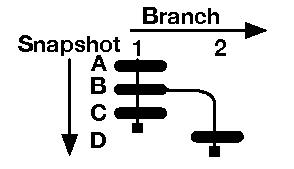
\includegraphics[width=55mm]{images/branches_paper}
\caption[Tree model]{Tree model: 2 branches and 4 snapshots: branch 1 contains the snapshots $A, B, C$; branch 2 contains the snapshot $D$;}
\label{fig:branches_simple}
\end{figure}


%Architecture details
A branch contains a sequence of snapshots but a snapshot can only belong to a single branch (Figure \ref{fig:branches_simple}). Each snapshot represents a possible version of the data item. A novel data item version is created only when the data item is written for the first time during each snapshot. Consequently, the data item may not have a version for each snapshot. Shuttle keeps a list of the versions in which each database item has been written (Section \ref{sec:arch:snapshot}).

%Problem of lack of versions:
For instance, in Figure \ref{fig:branches}, a data item $x$ may have the following sequence of versions on its version list: $[A,B,C,D,E]$. If $x$ has not been written in snapshot $E$, the version $E$ would not exists and the latest version of $x$ would be $D$. However, the snapshot $D$ has been compromised so it is not part of the current branch (branch 3). The latest non-tampered version of $x$ is the version $B$. If version $B$ does not exists, then the latest version is $A$.

%branch path
We define the concept of \emph{branch path}:  a Branch Path of a certain branch is the sequence of snapshots between the current snapshot and the root snapshot. A Branch Path of a certain branch defines the versions available to operations that belong to that branch. The branch path of branch $3$ in Figure \ref{fig:branches} is \{E, B, A\}. The one of branch $2$ is: \{D, C, B, A\}. When a branch is created, its branch path contains the its initial snapshot and the sub-sequence of snapshots in the branch path of the branch of the forked snapshot that are equal or previous to the forked snapshot.

%Version to read
The version accessed by an operation is defined using the branch path of the operation's branch and the version list of the accessed data item: operations read the latest version present in the \emph{version list} and in the \emph{branch path} and write the latest version in the branch path. Therefore, a new version, referring the initial snapshot of the new branch, is added to the version list on the first write operation to each data item during the replay.

%Isolation
This mechanism maps the operations to the correct versions and isolates the multiple, perhaps simultaneous, attempts to recovery the application without compromising the exposed application behavior. During the recovery process, users access the, perhaps corrupted, old branch loaded in the current computation and database instances. Therefore, the application remains online, perhaps with a degraded behavior, without exposing downtime to users.

%Working explanation and switching
At recovery time, the manager sends the new \emph{branch path} to every database instance. The new incoming users access the, perhaps corrupted, old branch while the requests being replace access the new branch. Therefore, the application remains online, perhaps with a degraded behavior, without exposing downtime to users. 

At some point, when the recovery is finishing, the user requests have to start being issued to the new branch. To do so, after replaying the requests, the proxy flag \emph{restraining} is set and every new request is marked with the \emph{restrain} flag. Database accesses marked with \emph{restrain} are delayed. After replaying the requests retrieved during the recovery process, the proxy sets the new branch in the subfield \emph{branch} of \ac{SRD} of the new requests, the \emph{restrain} flag is disabled and the database nodes are notified to proceed the accesses. This mechanism delays the processing of some requests, but this has typically a duration of seconds, compared with a recovery process that may take many minutes or even hours. 

This mechanism ensures the recovery phase to be finite. However, if the rate of requests being replayed is much higher than the rate of new requests, then the requests retrieved during the replay phase are also replayed without restraining new requests. Consequently, the restrain phase is shorter and required only to change branch. 

%Related work, advantages and example
While Aire \cite{retro} used a branching mechanism to perform a recovery process in various systems simultaneously, we propose the mechanism to isolate user accesses from the recovery process. Our model allows the tenants to select any snapshot as base to a new recovery process and create snapshots in different branches. Applications can contain multiple branches simultaneously. Figure \ref{fig:branches} represents an application with 3 branches: the branch 1 is the initial application branch where the tenant made three snapshots ($A$, $B$ and $C$). After detecting an intrusion, the tenant considered that snapshot $C$ is non-tampered and initiated a recovery process based on it creating the branch 2. Afterwards, the tenant made one snapshot ($D$) on branch 2. However, the snapshot $C$ is tampered. So the tenant initialized a novel recovery process based on snapshot $B$ creating the branch 3. In this scenario, the tenant would be unable to recover its application without the branching model. Since tenants may fork a new branch not only from the most recent snapshot. Therefore, the latest non-tampered version of a data item may not be its latest version.

\begin{figure}
\centering
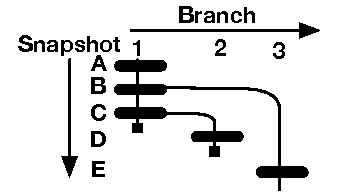
\includegraphics[width=65mm]{images/branches}
\caption[Tree model]{Tree model: 3 branches and 5 snapshots: branch 1 contains the snapshots $A, B, C$; branch 2 contains the snapshot $D$;  branch 3 contains the snapshot $E$.}
\label{fig:branches}
\end{figure}



Inactive snapshots and branches, for instance snapshot $D$ and branch 2 in Figure \ref{fig:branches}, can be deleted to reduce the used storage resources. In addiction, tenants can use the branching mechanism to test their intrusion recovery procedures in background, i.e, without exposing users to test issues.\\

If an intrusion happens during the replay phase, then its effects are stored in the branch of incoming requests. If the intrusion is detected before the restraining flag is set, then the malicious requests are not replayed in the new branch. Otherwise, tenants shall start another recovery process.\\





%%%%%%%%%%%%%%%%%%%%%%%%%%%%%%%%%%%%%%%%%%%%%%%%%%%%%%%%%%%%%%%%%%%%%%%%%%%%%%%%%%%%%%%%%%%%%%%%%%%%%%%%%%%%%%%%%%%%%%%%%%
\subsection{Non-determinism and consistency}
\label{sec:arch:consistency}

Shuttle provides an \ac{API} to handle nondeterminism and inconsistency cases.

%non-determinism: definition
An application is called nondeterministic if two subsequent executions with the same user input cannot be guaranteed to have the same have the same final state and outputs. Five of the main sources of non-determinism in \ac{PaaS} applications are: shared memory, thread concurrency, random number generation, timestamps and message exchanging.

%how non-determinism is handled
We assume requests to be independent thus they do not share memory and concurrent threads are independent. The \ac{API} of Shuttle provides a deterministic random number generation and a timestamp. It uses the \ac{RID}, which is a timestamp set by the proxy, as timestamp and pseudo-random number seed, so the replay of a request will use the same random numbers and timestamp. We consider a single timestamp per request to be enough for most applications. This mechanism is language independent. User requests and database accesses are ordered in a deterministic way using the operation list. Shuttle provides the following \ac{API} for the application developers:

\begin{enumerate}
  \item \textit{getTimestamp():} returns the timestamp (\ac{RID}) set by the proxy (\textit{long}).
  \item \textit{getRandomGenerator():} returns a random number generator that has \ac{RID} as seed.
\end{enumerate}

%User consistency
An important aspect of a recovery system like Shuttle is the application consistency seen by users. For instance, if an user does an action based on data written by a malicious action, which result of the user action replay is consistent. Since users have a non-deterministic behavior, they may have to be notified if a recovery took place and their data was modified. \\


%Related work
%In Undo for Operators \cite{undoForOperators}, operators must specify a compensation action for each request type. 
Since Shuttle is not tied to the application semantics, the actions to compensate the recovery process changes are unknown before the application is created. In addition, the application may contain client-side code, e.g., Javascript, that processes the application responses. For instance, a recover process reorders a list of items. The client-side code may sort the items so the list is seen ordered by users. A replay process taking into account the client-side consistency is proposed in \cite{warp}.


% Compensation API
Shuttle does not execute requests that returned an error in the first execution. We assume that requests are synchronous so users are immediately notified of the error and do not expect that the request will succeed in future. Similarly to other works in the area \cite{undoForOperators}, we assume that these cases are compensated by the user when they happen. As only requests that did not return an error are replayed, Shuttle considers an inconsistency when a request returns an error or a response is different during replay. Shuttle provides the following \ac{API} for the application programmer to define how inconsistencies are dealt with (Shuttle calls these functions in case they are launched by the tenant):

\begin{enumerate}
  \item \textit{preRecover():} invoked before the beginning of the recovery process.
  \item \textit{handleInconstency(request, previous response, new response, previous data items, new data items, action):} invoked when there is an inconsistency.
  \item \textit{postRecover(statistics, old version, new version):} invoked after the end of the recovery process.
\end{enumerate}

The first function allows tenants to perform a set of actions before the beginning of the recovery process, such as notifying the operations team or taking a new snapshot. 
The second function takes as input the operation that caused the inconsistency as well as the response and keys accessed during the normal execution and during the recovery process. It also takes as argument the action to take. Currently we consider three possible actions: 1) ignore the inconsistency; 2) notify the user of the inconsistency; 3) execute another request. This function is invoked, for instance, if a response during the replay is different than the response on the first request execution.
Using the \textit{postRecover} function, the tenant has access not only to the statistics of the recovery process but also to an interface to compare the database values before and after the recovery process and the application responses, before exposing the data to the users. 
Tenants can use this interface to notify their customer to verify their data.
%If tenants aim to determine if a request returned an error in the first execution due to an intrusion, Shuttle can replay the failed requests too.

%External consistency
Besides its users, an application may also interact with external services. We simplify the problem by considering that applications only obtain inputs from external services, disregarding the issue of outputs. The problem is treated in \cite{undoForOperators,aire}. Brown \textit{et al.} \cite{Brown_spheres} models each external service as a recoverable application. During the recovery phase, an external service can also be recovered if its input is distinct. Aire \cite{aire} proposes to initiate a recovery process in the external service and handles the inconsistencies of this process.


%%%%%%%%%%%%%%%%%%%%%%%%%%%%%%%%%%%%%%%%%%%%%%%%%%%%%%%%%%%%%%%%%%%%%%%%%%%%%%%%%%%%%%%%%%%%%%%%%%%%%%%%%%%%%%%%%%%%%%%%%%%%
% \subsection{System Administrator Support}
% \label{sec:arch:system_admin_support}

% Shuttle aims to facilitate the recovery process aiding the tenants to recover their applications from intrusions. Shuttle helps the tenant to identify the malicious requests based on: 
% \begin{enumerate}
% \item tainted responses;
% \item the requests that accessed a set of data items;
% \item per user, per user session, per ip-range
% \end{enumerate}
% %    \hl{a maquina que foi afectada, tracking do codigo que foi actualizado, etc ha muitos criterios possiveis}.

%  It also displays the requests dependency graph. It allows the tenant to preview the results of the recovery process without exposing them to the users. It provides a database version compare tool to check if the vulnerability is correctly mitigated.
% \hl{apago esta secção?}

%%%%%%%%%%%%%%%%%%%%%%%%%%%%%%%%%%%%%%%%%%%%%%%%%%%%%%%%%%%%%%%%%%%%%%%%%%%%%%%%%%%%%%%%%%%%%%%%%%%%%%%%%%%%%%%%%%%%%%%%%%%%
\subsection{Full and Selective Replay}
\label{sec:arch:selective_replay}

%Full vs selective goals
We propose two approaches for intrusion recovery: full replay and selective replay. Full replay consists in replaying every request done after the  snapshot. Executing many requests takes considerable time, so this approach is adequate for intrusions detected reasonably fast after they happen, e.g., a few days. 


%Explain
Selective replay (Section \ref{sec:related:recovery_models})  re-executes only part of the requests so it is faster than full-replay. However, it requires tenants to provide a set of malicious actions (i.e., requests) $A_{intrusion}$. This set is used to deduce the set of tainted requests $A_{tainted}$. A request is said to be tainted if it is one of the attacker’s requests or if it reads objects written by tainted request \cite{taser,itdb,phoenix}.  

%Tait
Tainted requests can also be determined by Shuttle considering the tampered data items and an estimated intrusion moment. Selective replay approach loads only the previous versions of the tainted objects, $O_{tainted}$, and replays only the legitimate operations, which were tainted, $A_{tainted} \notin A_{intrusion}$, to update the application persistent state. Selective replay, as compensating actions, does not remove the effects of unlogged actions because their dependencies are unknown. 

%related work
In \cite{goel,retro}, the set of tainted operations, $A_{tainted}$, is determined using \textit{taint propagation via replay}. To do so, they load a previous version, from a snapshot, of the objects in $O_{intrusion}$. Then, the actions, which are dependent from the restored objects, are replayed and their output objects are updated. The forward actions, which depend on the updated objects, are also replayed while their inputs are different from the first execution. The propagation is done thought the output of actions with different execution.
Unlike these approaches, Shuttle does not store the input and output of every action, i.e., database operation. Shuttle proposes an approach in which the requests are replayed, at least, until the first snapshot after the selected snapshot. Consequently, the application semantic must remain unchanged, i.e., the same request and same input must perform the same write operations. Otherwise, the dependencies between requests are unpredictable and the tainted requests can not be determined. An approach that allows to update the application semantics is proposed in \cite{warp}. We consider storing all versions of a data item has prohibitive storage costs for enterprise applications.\\

%Which requests are replayed?
For instance, consider the dependency graph of Figure \ref{fig:selectiveGraph}, in which every request reads a data item and writes a new value on the same data item. The request $4$ was identified as a malicious request. Therefore, requests $5,6,7,8$ are tainted. Since Shuttle does not keep every version of the entries, the value read by request 4 is unknown. In order to get this value, Shuttle must replay the {req.~2}, which wrote the value read by {req.~4}. The value read by request 2 is known because Shuttle performed the checkpoint A. Since the application semantics remains the same and its input is known, {req.~3} does not need to be replayed. Requests $5,6,7$ are replayed since they depend on the malicious {req.~4}. Values read by request 8 are known due to checkpoint B. Therefore, {req.~8} may not be executed if the value of the data items remains the same. Shuttle performs \textit{taint via-replay}: if a request writes in a data item which were not written previously, then the requests which read or write that data item, are also replayed. For instance, the {req.~9} may read a data item written by the {req.~4} during the replay but not during its first execution.\\


\begin{figure}
\centering
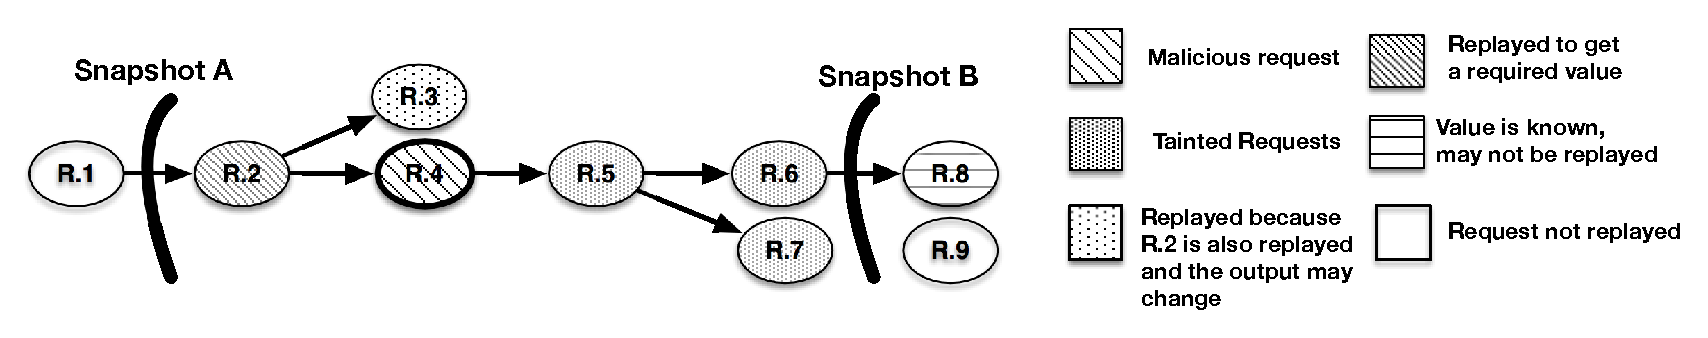
\includegraphics[width=150mm]{images/selectiveDependency_legended}
\caption[Dependency graph]{Dependency graph: $R.1$ is previous to a snapshot $A$; $R.3$ is dependent on $R.2$, which is replayed to get the read values; $R.4$ is a malicious request; $R.5,R.6,R.7$ are tainted; $R.8$ may not be replayed; $R.9$ is independent of the rest}
\label{fig:selectiveGraph}
\end{figure}

The selective replay process is as follows (full replay is simpler so we skip it):
\begin{enumerate}
\item \textit{Determine the malicious requests $A_{intrusion}$.}
Based on initial data such as user session compromised or data items accessed or other criteria, the tenant determines the requests $A_{intrusion}$ used by the attacker to compromise the application. For instance, $A_{intrusion} = \{R.4\} $ in Figure \ref{fig:selectiveGraph}.

\item \textit{Use $A_{intrusion}$ to determine the set of tainted requests $A_{tainted}$.}
For each request in $A_{intrusion}$, traverse the dependency graph in causality order and add these nodes to $A_{tainted}$ (in the figure $A_{tainted} = \{R.5,R.6,R.7,R.8\}$).


\item \textit{Get the requests needed to obtain the values read by $A_{tainted}$ and their effects.} 
Instead of storing the input and output of every action or versions of every data item, we propose to replay the actions which $A_{tainted}$ depends on. The data item value is known at the snapshot instant so the algorithm transverses the graph in inverse causality order from each request in $A_{tainted}$ and stores the requests in $A_{replay}$ ($A_{replay} = \{R.2\} \cup A_{tainted}$). $A_{replay}$ is expanded by traversing the graph from each of its elements on causality order to determine the requests which can be affected by the re-execution of $A_{replay}$ ($A_{replay} = A_{replay} \cup R.3$). Requests subsequent to the first snapshot after the latest malicious request may not be repeated as the data item version is known (version read by $R.8$ is stored in snapshot B).

\item \textit{Determine the replay order.} 
The set $A_{replay}$ is sorted on non-clustered \emph{start-end order}.

\item \textit{Load the previous data item versions}
Shuttle loads the version in the selected snapshot of the data items read by the requests in $A_{replay}$ and written by $A_{malicious}$.

\item \textit{Replay the requests}
Requests in $A_{replay}$ are replayed. If an access is not contained in operation list, then a new dependency is established and the requests that accessed the data item during the first execution are also replayed as in \emph{taint propagation via replay} \cite{retro}. For instance, $R.9$ is replayed if it reads an item written during recovery process but not during normal execution. 
\end{enumerate}

%merging branches
%After replaying the tainted requests, Shuttle compares the branches. \hl{ver se isto é necessário, na prática pode carregar apenas os dados novos}
% Depois para fazer o merge: compara as branches indo de key em key e comparando o hash dos valores guardados. As combinações são:
% |  Old  |   Recuperada |
%    A            A           - (sao iguais) - está tudo bem, um algoritmo de compressão pode colocar ambas as versões a apontar para o mesmo valor
%    -            B           - (nova entrada) - A versão recuperada ganha
%    A            B           - (modificado) - A versão recuperada ganha

% As entradas recuperadas escrevem sobre as que existem. Neste caso, os items apagados são também apagados.


 %A eficacia e melhoramento do selective replay depende do numero de entradas afectadas. Um simulador foi implementado e os resultados sao apresentados nos testes.

 Shuttle does not require generating a dependency graph in non-clustered full replay mode. The dependency graph is required in the case of clustered full replay to identify the independent clusters of requests and on selective replay to determine the tainted requests. We use the database operation lists to create the dependency graph and to order the execution of parallel requests without knowledge of the application protocol. 
 
 In summary, the selective replay approach reduces the number of requests to be replayed during the recovery process but implies that the application remains unchanged and does not revert the actions performed by unlogged requests. 


%%%%%%%%%%%%%%%%%%%%%%%%%%%%%%%%%%%%%%%%%%%%%%%%%%%%%%%%%%%%%%%%%%%%%%%%%%%%%%%%%%%%%%%%%%%%%%%%%%%%%%%%%%%%%%%%%%%%%%%%%%%%
\section{Chapter Summary}
\label{sec:arch:summary}
Shuttle recovers from security intrusions loading a previous snapshot and replaying the legitimate requests. It uses database snapshot and clustering to reduce the recovery time. Shuttle leverages the pay-per-usage model of \ac{PaaS} to provide a cost-efficient and fast recovery service instantiating the replay instances and more application containers on demand during the recovery process. \\

Shuttle proposes two approaches to perform replay: selective replay and full replay. 

\begin{table}[h]
\centering
    \begin{tabular}{l|ll}
               & Clustering & Non-Clustering \\ \hline
    Selective &  \xmark     &  \cmark        \\
    Full      &  \cmark     &  \cmark             
    \end{tabular}
\caption{Shuttle Replay modes}
\label{tab:operation_types}
\end{table}

The full replay approach supports parallel re-execution of requests that belong to independent clusters (clustering). Clustering is not supported on selective replay because the \textit{taint propagation via replay} defines the set of requests to replay at running time. Clustering is not supported with selective replay because taint propagation via replay defines the set of requests to be replayed in runtime.

The decentralized applications are more vulnerable to failures because of the single proxy architecture. However, we argue that future architectures can consider replication of the proxy, load balancer, Shuttle Storage and database. 